The Standard Model (SM) of particle physics has been very successful at describing the interactions of fundamental particles. With the discovery of the Higgs boson, the SM is complete and may be the correct theory up to the energy scale of gravity. The Large Hadron Collider (LHC) was built in order to probe this. The SM and look for solutions to some of the unknown issues in particle physics that may involve physics beyond the SM.

Despite the overwhelming success of the SM, some uncertainty remains in predictions in the Quantum Chromodynamics (QCD) sector. Due to its non-pertubative nature, QCD has not been as precisely measured as other parts of the SM. In particular, since the top quark was only discovered in the late 1990s, its decays and properties have not been as studied as thoroughly. 

The top quark plays a special role in the SM and in searches for
physics beyond the SM .  Its large mass means its coupling to the
Higgs Boson is large.  This high mass, together with the presence of 
charged leptons, missing energy and $b$-jets as top decay products,
make the top a primary source of background in many searches for new physics.
For these reasons, accurate modeling of the properties of top quark
events is an important part of the LHC program.

Measurements of the activity of additional jets (jets not coming from the decay of top quarks)
have been made by ATLAS~\cite{gapfraction,hdamp,ljets} and CMS\cite{Chatrchyan:2014gma} using
pp data with $\sqrt{s}=7~\TeV$.  Comparison of the measured distributions with the predictions of Monte Carlo (MC) generators
indicate that some state-of-the-art generators (e.g. \textsc{MC@NLO}) have a difficult time in reproducing the data,
while for others  agreement with data can be improved with appropriate
choice of generator parameters.  For example, in \textsc{Powheg+Pythia} adding a damping
function that limits the resummation of higher-order effects incorportated into  the Sudakov form factor improves
the agreement between data and MC~\cite{hdamp} at 7~TeV.  

The range of predictions observed in standard MC generators for
8~\TeV\ $pp$ interactions is shown in 
Figure~\ref{fig:introtjets}. The fiducial definition of these extra jets is provided in Chapter~\ref{ch:extrajets}.  
Differences in rate as large as 40\%\  are seen for
jet multiplicities $\ge 5$.  Differences up to 20\%\ for the leading
jet and up to 40\%\ for the subleading jet are seen at high jet transverse
momentum.  
\begin{figure}
\centering
\subfloat{
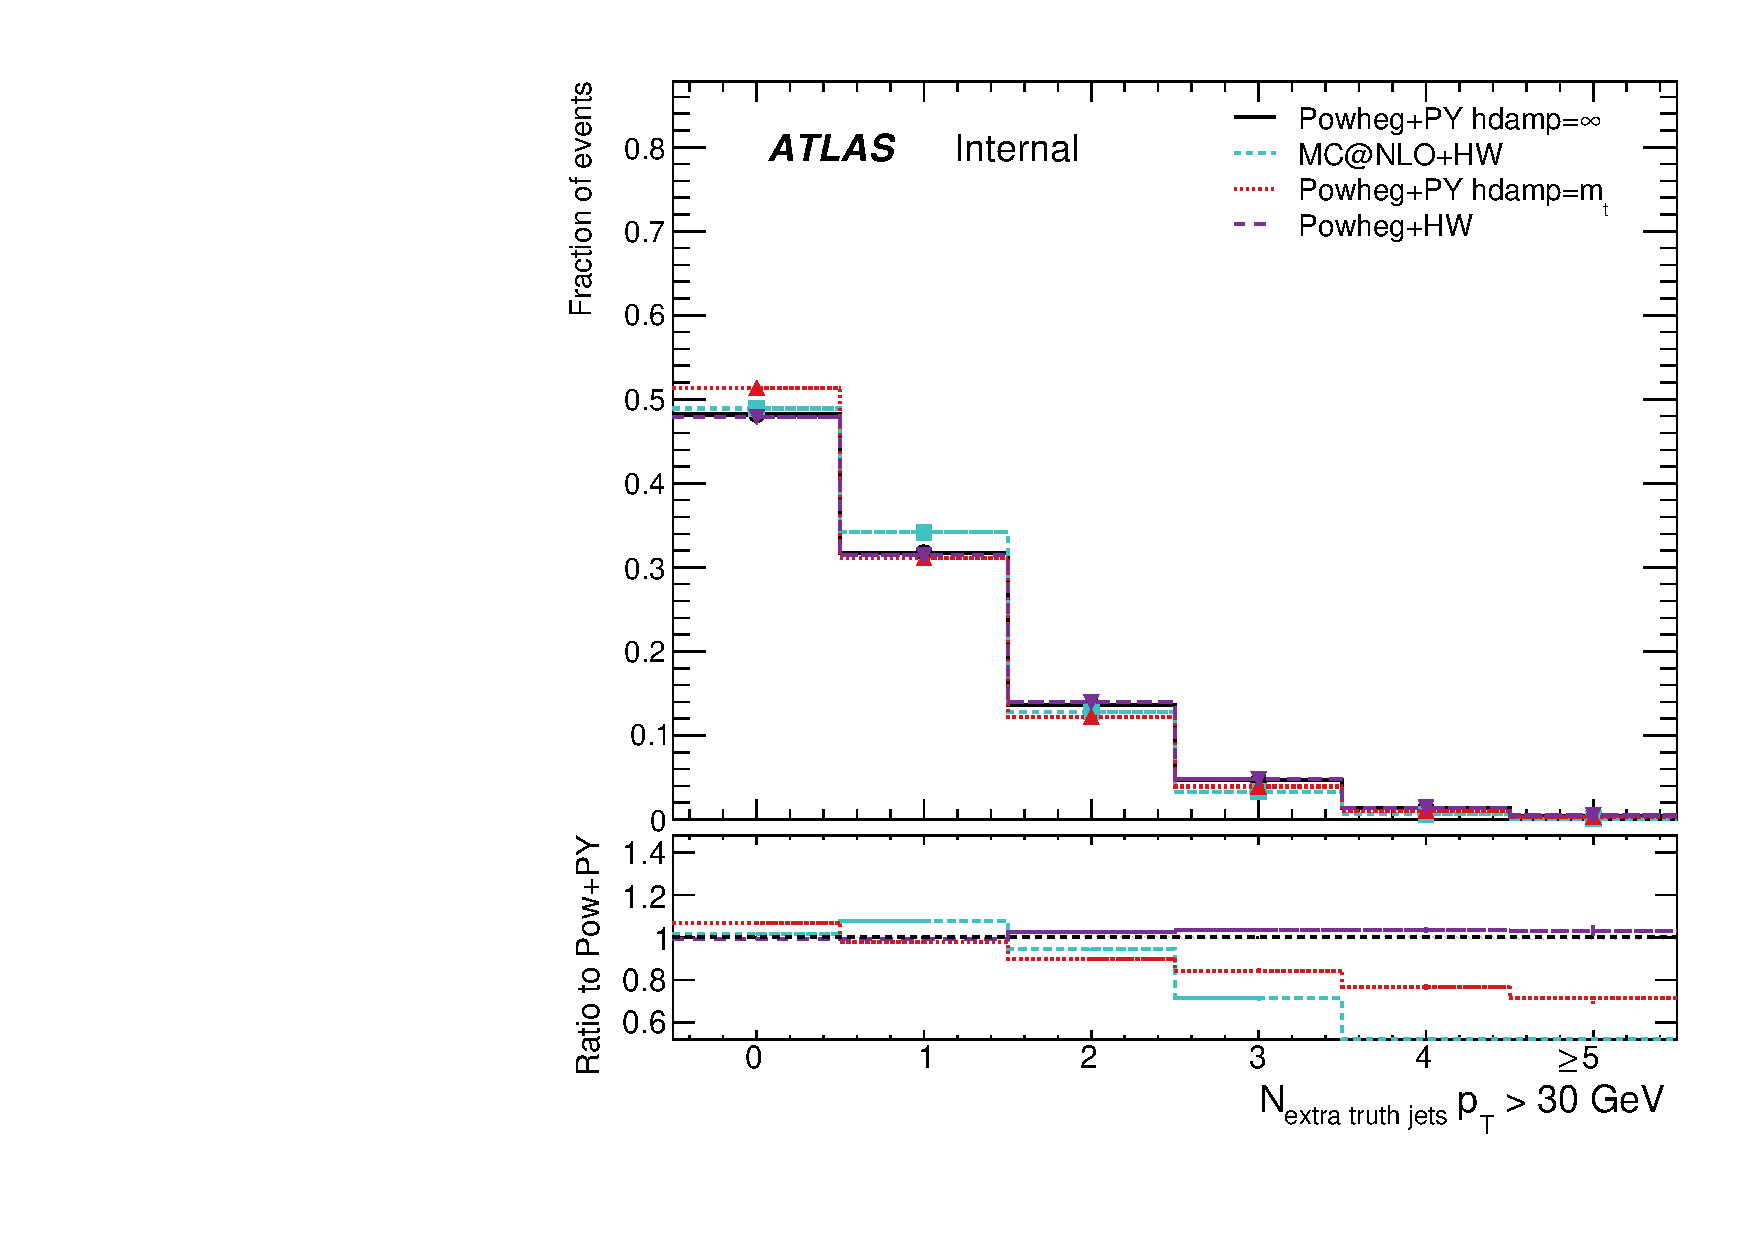
\includegraphics[width=0.45\textwidth]{fig/MCComp/NTruthExtraJets30.pdf}}
~
\subfloat{
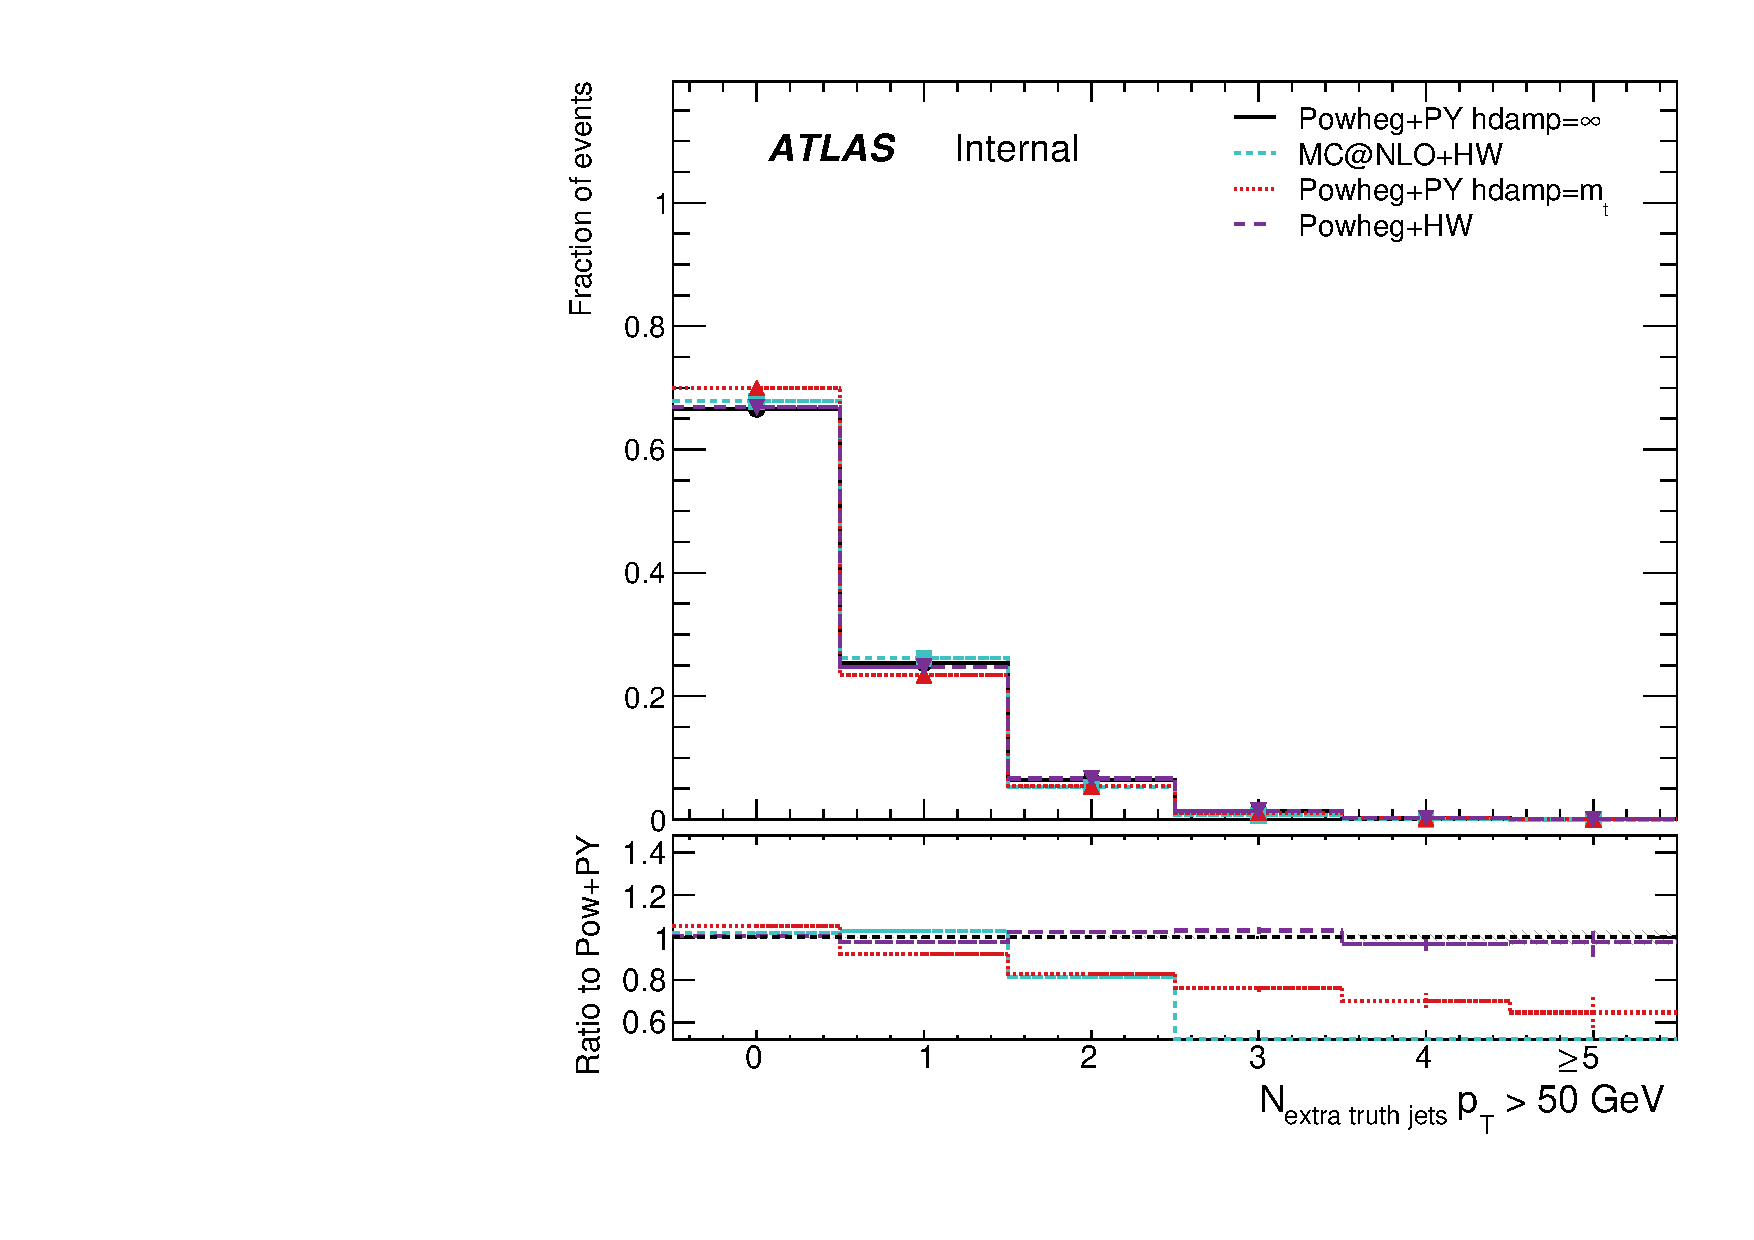
\includegraphics[width=0.45\textwidth]{fig/MCComp/NTruthExtraJets50.pdf}} \\
\subfloat{
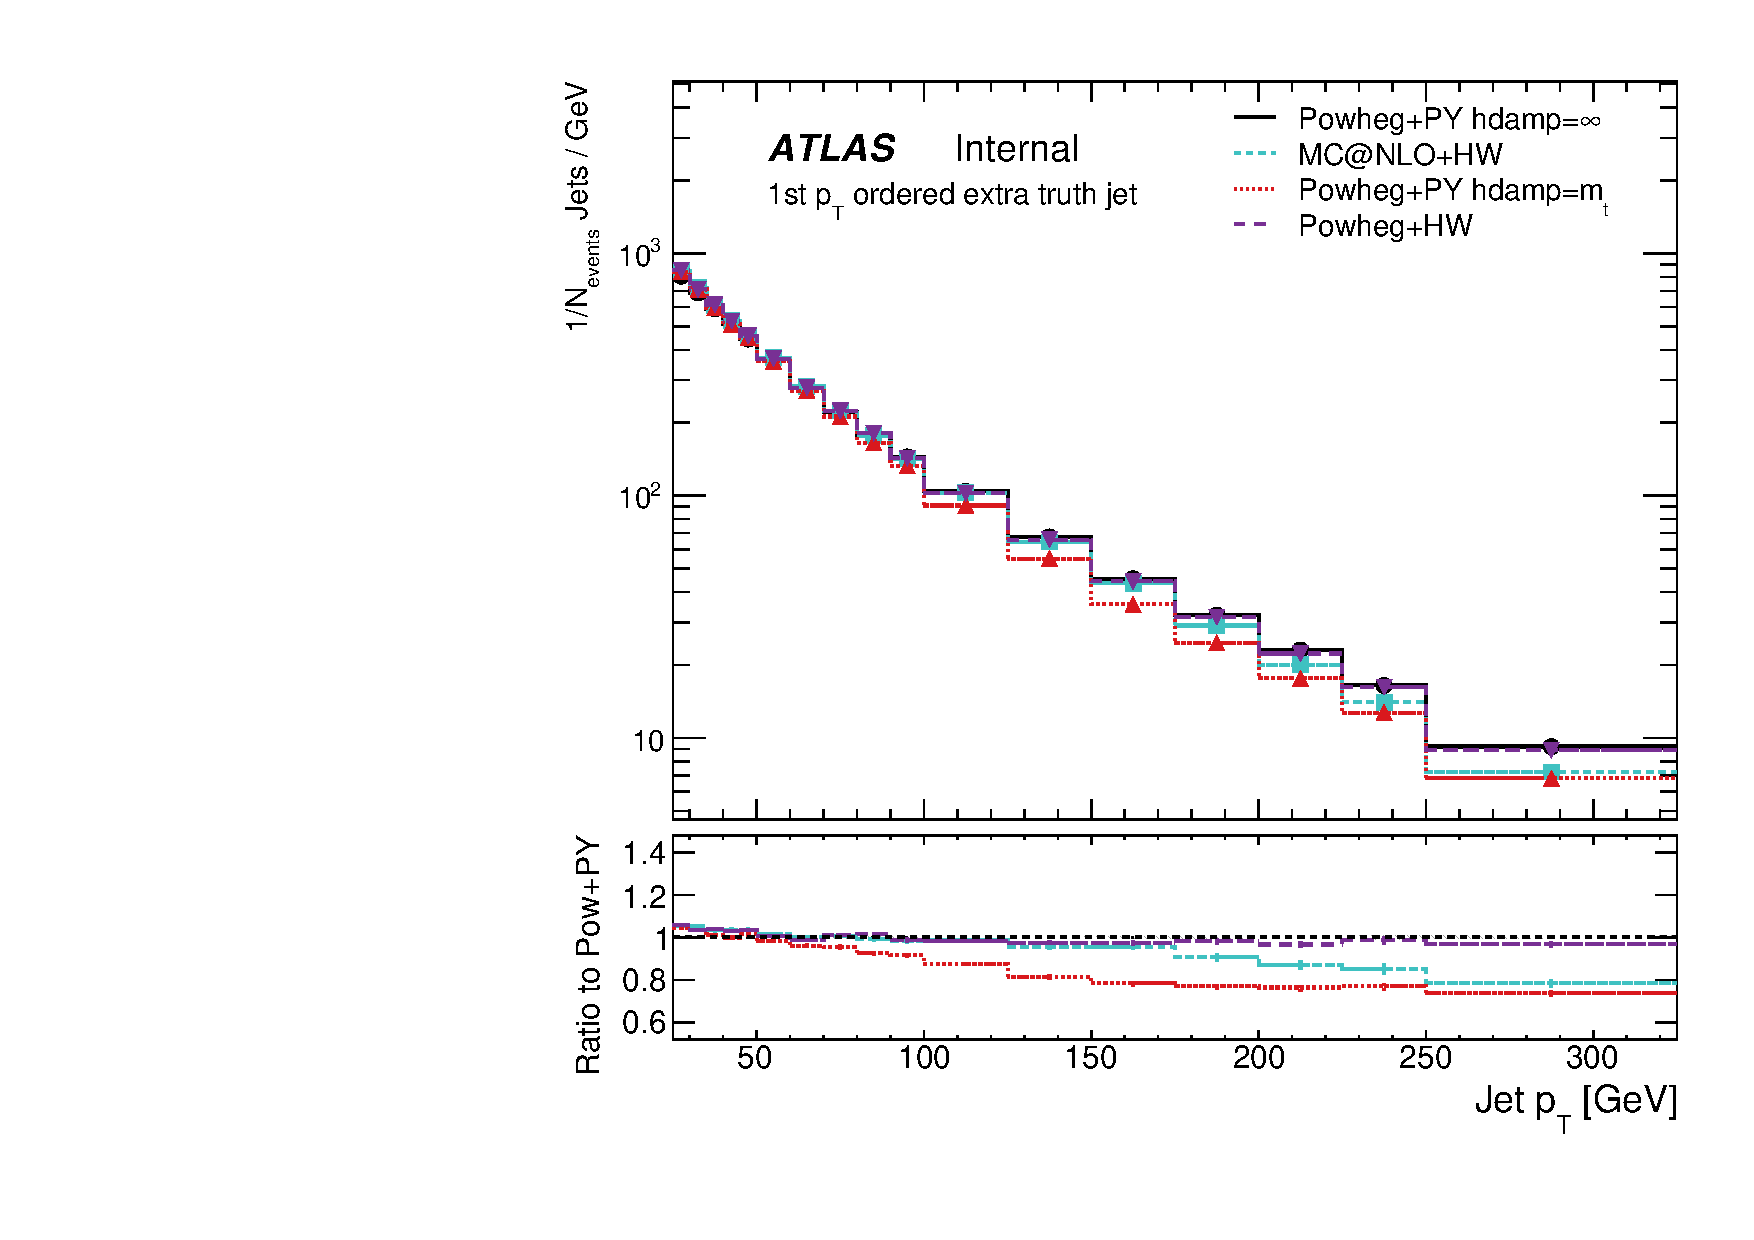
\includegraphics[width=0.45\textwidth]{fig/MCComp/TruthPtJet0.pdf}} ~
\subfloat{
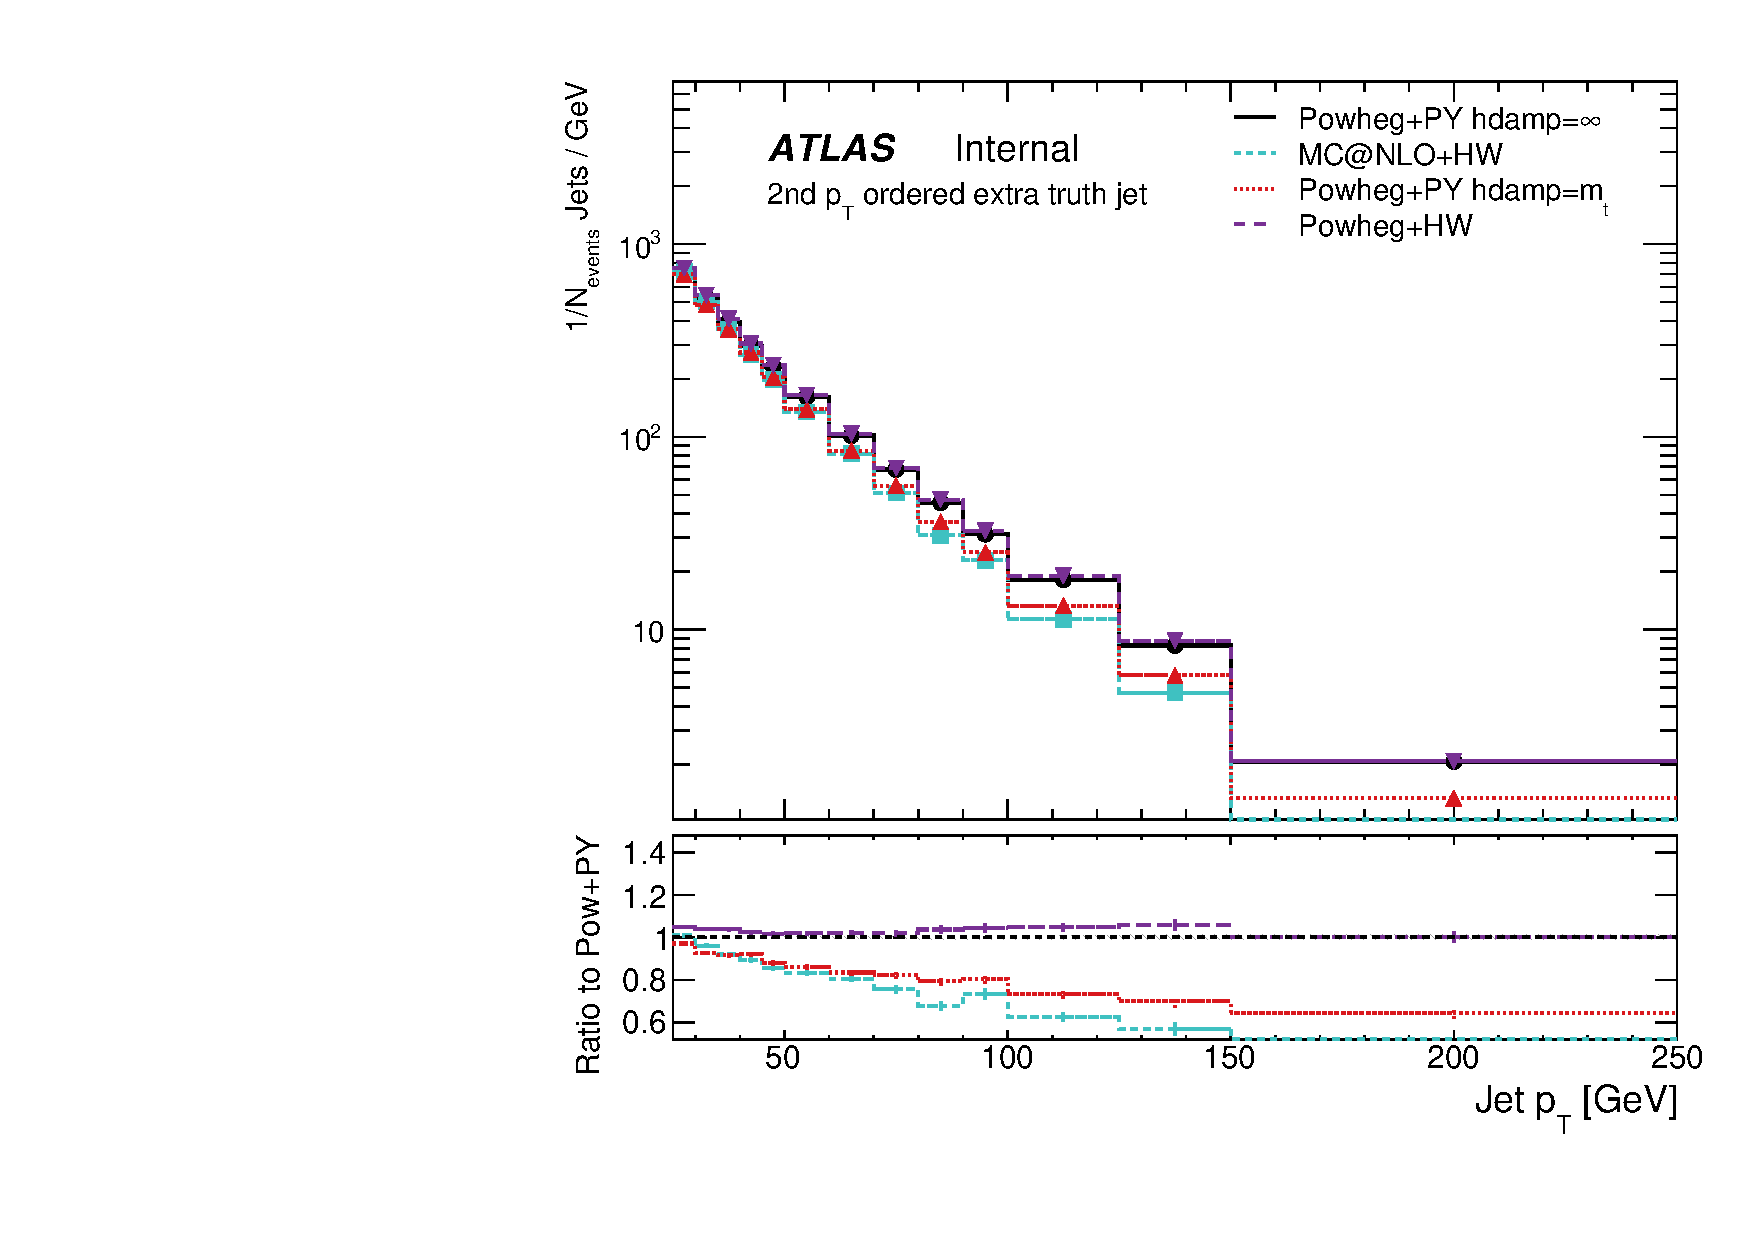
\includegraphics[width=0.45\textwidth]{fig/MCComp/TruthPtJet1.pdf}}
\caption{Comparison of the truth level extra jet multiplicity and $\pt$ distributions in generated $\ttbar$ events with an opposite-sign $e\mu$ pair and at least 2 $b$-jets.  Jets are reconstructed using the anti-$k_t$ algorithm with 
the distance parameter $R=0.4$.
Each simulation is normalized by the number of events passing the truth-level selection.
The ratio plots compare each generator to the predictions of the baseline \textsc{ Powheg+Pythia} sample with the hdamp parameter
set to $\infty$.}
\label{fig:introtjets}
\end{figure}

This analysis presents a study of jet activity in top quark events using the $e\mu$ final state 
with at least 2 $b$-tagged jets in $pp$ collisions at $\sqrt{s}=8$ TeV. The analysis employs
an event selection which closely matches that used in the ATLAS 8~\TeV\ cross
section measurement\cite{xsec}.
The particle-level fiducial cross section \sigmapti\ for additional jets with 
rank 1-4, where rank=1  is the leading additional jet are measured and
these distributions are used to obtain the extra jet multiplicity as a function of minimum jet \pt\ threshold. 

This thesis is structured as follows: FINAL CHAPTER STRUCTURE TO FOLLOW